%%%%%%%%%%%%%%%%%%%%%%%%%%%%%%%%%%%%%%%%%%%%%%%%%%%%%%%%%%%%%%%%%%%%%%%%%%%%%%%%
% experiment.tex: Chapter describing the experiment
%%%%%%%%%%%%%%%%%%%%%%%%%%%%%%%%%%%%%%%%%%%%%%%%%%%%%%%%%%%%%%%%%%%%%%%%%%%%%%%%
\chapter{\gls{ldmx-full}}
\label{chapter:ldmx:experiment}

\gls{ldmx} is a proposed fixed-target experiment aiming to definitively explore
the light dark matter phase space. Even as a proposed experiment, it has a detailed
plan for construction, a beam already in construction, and well established connections
with current technologies used within \gls{hep}. While \gls{ldmx} is not yet built,
it has a well formulated simulation infrastructure that can realistically model
how the detector design responds to various types of interactions happening within it.

\section{The Beam Line}
LCLSII \cite{lcls-ii} and LESA \cite{lesa-design}

\section{Detector Design}
LDMX is a missing momentum experiment and its design is focused on measuring
\emph{both} the incoming and outgoing momenta of charged particles interacting
with a thin target.
This design has led to four subsystems with LDMX each with specialized roles.
\begin{enumerate}
    \item \textbf{Trigger Scintillator} Count the number of electrons incident on the target.
    \item \textbf{Tracker} Measure charged particle momenta both before (``Tagger'') and after (``Recoil'') the target.
    \item \textbf{Electromagnetic Calorimeter} (ECal) Measure the total energy of electrons, positrons, and photons.
    \item \textbf{Hadronic Calorimeter} (HCal) Veto additional particles difficult for other subsystems to measured (muons, pions, hadrons,...).
\end{enumerate}
\cref{fig:ldmx-det} displays these subsystems in a diagram along with a representation of
a dark brem interaction occurrring within the target.

\begin{figure}
    \centering
    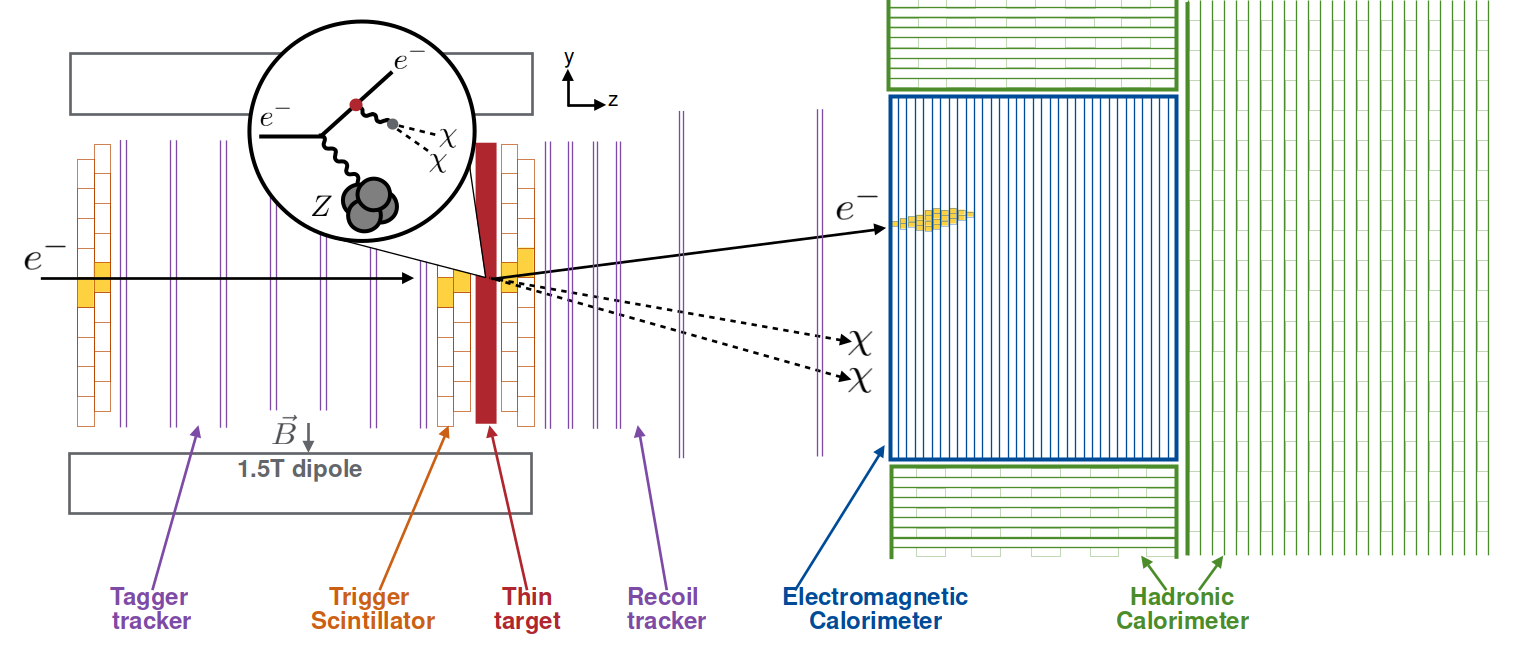
\includegraphics[width=0.9\textwidth]{figures/ldmx/experiment/detector.png}
    \caption{
        Diagram of LDMX detector apparatus with a representation of a signal event where
        a dark brem occurs within the target. Diagram is not to scale. Credit to Christian Herwig
        for original development of diagram.
    }
    \label{fig:ldmx-det}
\end{figure}

\section{ECal}
More detail about ECal since it relates to the ME search later.

\begin{figure}
    \centering
    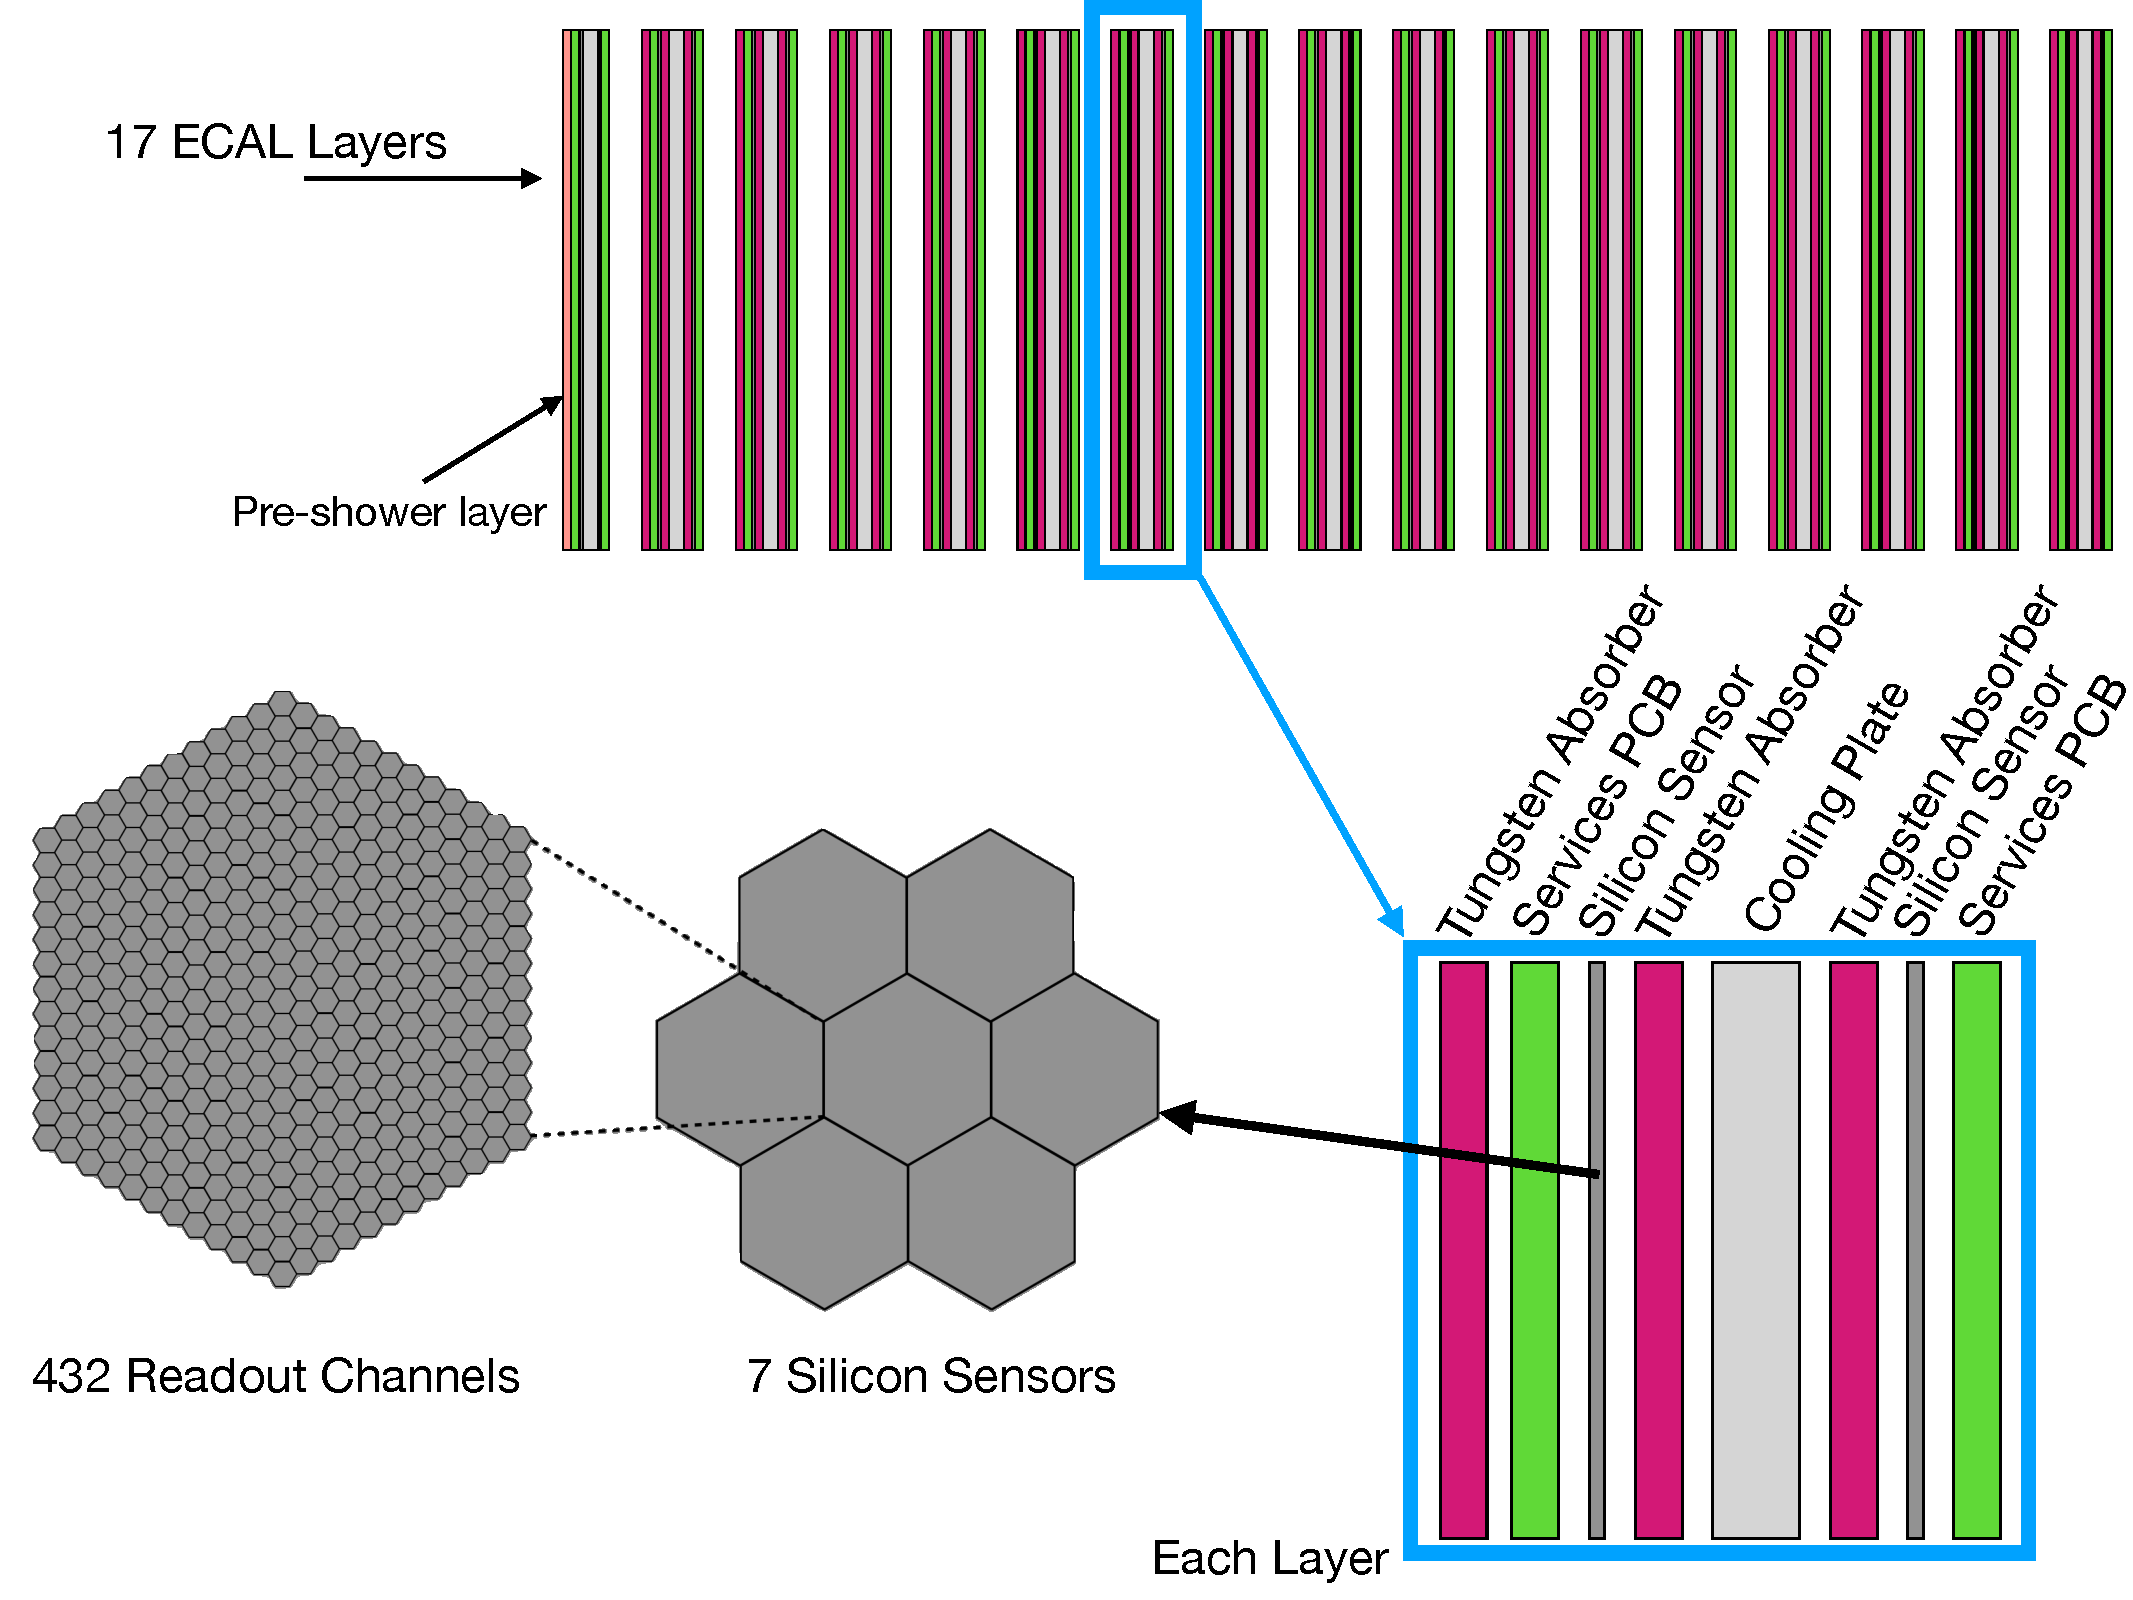
\includegraphics[width=0.9\textwidth]{figures/ldmx/experiment/ecal.pdf}
    \caption{
        Diagram of LDMX ECal construction showing the longitudinal segmentation
        (top and bottom right) and the transverse segmentation (bottom left).
        Credit to Joe Muse.
    }
    \label{fig:ldmx-ecal}
\end{figure}
%%%%%%%%%%%%%%%%%%%%%%%%%%%%%%%%%%%%%%%%%%%%%%%%%%%%%%%%%%%%%%%%%%%%%%%%%%%%%%%%
